\newpage
\subsection{Precision}
    Following are the precision @ i curves. Graphs in the first column are for OCMFH\cite{ocmfh} on two different datasets with fixed bit vector length(16). Graphs in the second column compares the precision value on varying bit vector length for OCMFH\cite{ocmfh} on nuswide dataset.
        \begin{figure}[H]
            \begin{minipage}[!h]{0.6\linewidth}
                \centering
                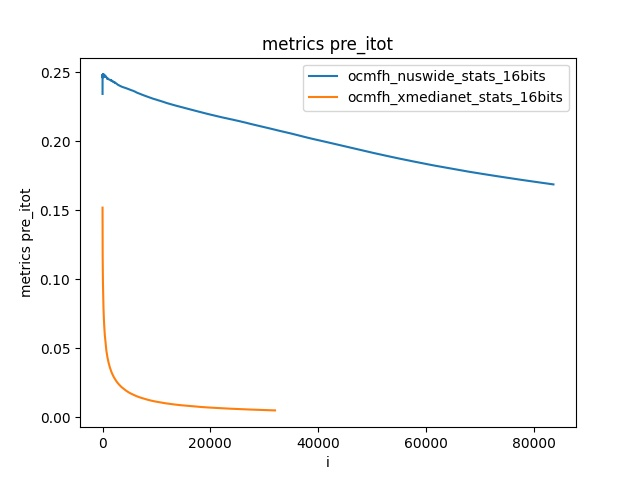
\includegraphics[width=\linewidth]{resultsImages/precision/metrics pre_itot_ocmfh_both.jpeg}
                % \caption{Query type: min}
                % \label{fig:six_core_min}
                % \vspace{0.1ex}
                % \hspace{0ex}
            \end{minipage}
            \begin{minipage}[!h]{0.6\linewidth}
                \centering
                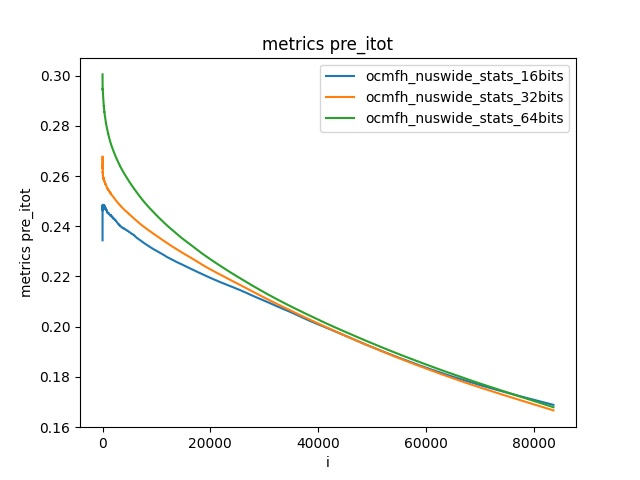
\includegraphics[width=\linewidth]{resultsImages/precision/metrics pre_itot_ocmfh_nuswide.jpeg}
                % \caption{Query type: sum}
                % \label{fig:six_core_sum}
                % \vspace{0.1ex}
                % \hspace{0ex}
            \end{minipage}
            \begin{minipage}[!h]{0.6\linewidth}
                \centering
                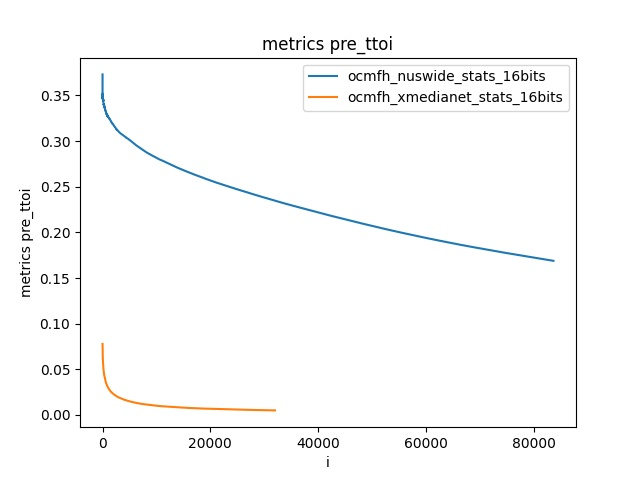
\includegraphics[width=\linewidth]{resultsImages/precision/metrics pre_ttoi_ocmfh_both.jpeg}
                % \caption{Query type: countrange}
                % \label{fig:six_core_countrange}
                % \vspace{0.1ex}
                % \hspace{0.1ex}
            \end{minipage}
            \begin{minipage}[!h]{0.6\linewidth}
                \centering
                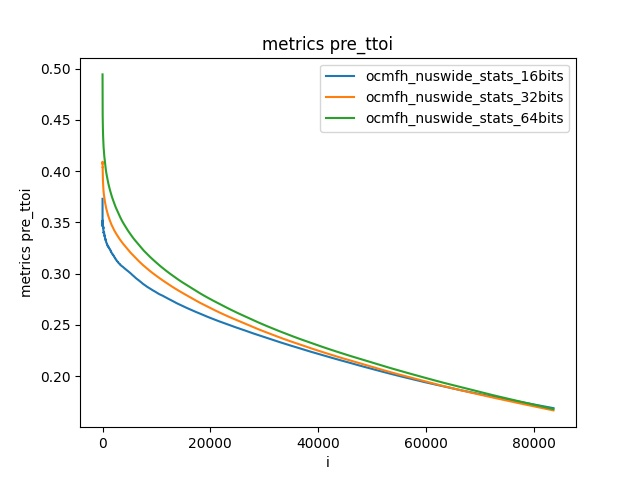
\includegraphics[width=\linewidth]{resultsImages/precision/metrics pre_ttoi_ocmfh_nuswide.jpeg}
                % \caption{Query type: max}
                % \label{fig:six_core_max}
                % \vspace{0.1ex}
                % \hspace{0.1ex}
            \end{minipage}
        \caption{Precision metric for OCMFH on various datasets}
        \label{fig:}
        \end{figure}
        \FloatBarrier